\documentclass[10pt,
  aspectratio=169,
  serif,
  mathserif,
  professionalfont,
  compress,
  handout,
  % table,
  % svgnames
  ]{beamer}\usepackage[]{graphicx}\usepackage[]{color}
% maxwidth is the original width if it is less than linewidth
% otherwise use linewidth (to make sure the graphics do not exceed the margin)
\makeatletter
\def\maxwidth{ %
  \ifdim\Gin@nat@width>\linewidth
    \linewidth
  \else
    \Gin@nat@width
  \fi
}
\makeatother

\definecolor{fgcolor}{rgb}{1, 1, 0.941}
\newcommand{\hlnum}[1]{\textcolor[rgb]{0.804,0.718,0.71}{#1}}%
\newcommand{\hlstr}[1]{\textcolor[rgb]{0.604,0.753,0.804}{#1}}%
\newcommand{\hlcom}[1]{\textcolor[rgb]{0.439,0.502,0.565}{#1}}%
\newcommand{\hlopt}[1]{\textcolor[rgb]{1,1,0.941}{#1}}%
\newcommand{\hlstd}[1]{\textcolor[rgb]{1,1,0.941}{#1}}%
\newcommand{\hlkwa}[1]{\textcolor[rgb]{0.941,0.902,0.549}{#1}}%
\newcommand{\hlkwb}[1]{\textcolor[rgb]{1,0.871,0.678}{#1}}%
\newcommand{\hlkwc}[1]{\textcolor[rgb]{0.545,0.941,0.702}{#1}}%
\newcommand{\hlkwd}[1]{\textcolor[rgb]{0.545,0.941,0.902}{#1}}%
\let\hlipl\hlkwb

\usepackage{framed}
\makeatletter
\newenvironment{kframe}{%
 \def\at@end@of@kframe{}%
 \ifinner\ifhmode%
  \def\at@end@of@kframe{\end{minipage}}%
  \begin{minipage}{\columnwidth}%
 \fi\fi%
 \def\FrameCommand##1{\hskip\@totalleftmargin \hskip-\fboxsep
 \colorbox{shadecolor}{##1}\hskip-\fboxsep
     % There is no \\@totalrightmargin, so:
     \hskip-\linewidth \hskip-\@totalleftmargin \hskip\columnwidth}%
 \MakeFramed {\advance\hsize-\width
   \@totalleftmargin\z@ \linewidth\hsize
   \@setminipage}}%
 {\par\unskip\endMakeFramed%
 \at@end@of@kframe}
\makeatother

\definecolor{shadecolor}{rgb}{.97, .97, .97}
\definecolor{messagecolor}{rgb}{0, 0, 0}
\definecolor{warningcolor}{rgb}{1, 0, 1}
\definecolor{errorcolor}{rgb}{1, 0, 0}
\newenvironment{knitrout}{}{} % an empty environment to be redefined in TeX

\usepackage{alltt}

% Tamanho de fonte e distância entre linhas.
\renewenvironment{knitrout}{
  \renewcommand{\baselinestretch}{0.75}%\tiny
}{}

%-----------------------------------------------------------------------
% Pacotes padrões.

% Fontes.
\usepackage{palatino}
\usepackage{eulervm}
\usepackage{inconsolata}

% Esses pacotes dão clash.
% http://tex.stackexchange.com/questions/51488/option-clash-with-xcolor-and-tikz
% \usepackage{xcolor} %% opções no \documentclass{} para evitar clash.
% \definecolor{mycolor}{rgb}{0.13,0.53,0.53}
% \definecolor{mycolor2}{rgb}{0.725,0,0.18}

\usepackage{hyperref}
% \hypersetup{colorlinks, allcolors=., urlcolor=structure}
% \hypersetup{colorlinks}

\usepackage[brazil]{babel}
\usepackage[utf8]{inputenc}
\usepackage{graphicx}
\usepackage{amsmath, amsfonts, amssymb, amsxtra, amsthm, icomma}
\usepackage{geometry, calc, setspace, indentfirst}
% \usepackage{colortbl}
\usepackage{enumerate}
\usepackage{float}

\usepackage[hang]{caption}
\captionsetup{font=footnotesize,
  labelfont=footnotesize,
  labelsep=period}

% Listas em duas colulas.
\usepackage{multicol}
\newenvironment{itemize2}{%
  \vspace*{-1em}
  \begin{itemize}
    \begin{multicols}{2}
    }{%
    \end{multicols}
  \end{itemize}
}

% Texto no corpo do beamer justificado.
\usepackage{ragged2e}
\justifying

%-----------------------------------------------------------------------

% A lot of options:
% http://latex-community.org/forum/viewtopic.php?f=55&t=17646
\useoutertheme[
  width=60pt,
  height=30pt,
  right,
  hideothersubsections
  ]{sidebar}

\makeatletter
\setbeamertemplate{caption}[numbered]
\setbeamertemplate{section in toc}[sections numbered]
\setbeamertemplate{subsection in toc}[subsections numbered]
\setbeamertemplate{sections/subsections in toc}[ball]{}
\setbeamertemplate{section in sidebar right}[sections numbered]
\setbeamertemplate{frametitle continuation}{\gdef\beamer@frametitle{}}
\setbeamertemplate{navigation symbols}{} %% Retira a barra de navegação.
% \setbeamertemplate{blocks}[rounded][shadow=FALSE]
% \setbeamercolor{block title}{fg=structure, bg=mycolor!20!white}
\makeatother

% Frames com sessão e/ou subsessão.
\addtobeamertemplate{frametitle}{
  \let\insertframetitle\insertsubsectionhead}{}
\makeatletter
\CheckCommand*\beamer@checkframetitle{
  \@ifnextchar\bgroup\beamer@inlineframetitle{}}
\renewcommand*\beamer@checkframetitle{
  \global\let\beamer@frametitle\relax\@ifnextchar\bgroup
  \beamer@inlineframetitle{}}
\makeatother

%-----------------------------------------------------------------------
% Comandos.

\newcommand{\n}[1]{\textbf{#1}}

%-----------------------------------------------------------------------

\AtBeginSection[]{
  \begin{frame}[c,allowframebreaks]
    \begin{center}
      {\thesection} \\ \vspace{0.3cm}
      \parbox{0.6\textwidth}{
        \centering {\Large \textcolor{structure}{\insertsection}}}\\
    \end{center}
  \end{frame}
}

%-----------------------------------------------------------------------
% Definições dos proprietários.

\title[MANOVA]{
  \LARGE Análise de Variância Multivariada \\ para Dados Não Gaussianos \\ via Teste Wald}


\subtitle{Uma visão geral}


\author[Lineu Alberto]{%\small
  Lineu Alberto Cavazani de Freitas \\
  \texttt{lineuacf@gmail.com}
}

\institute[UFPR]{
  PPG Informática \\
  Data Science \& Big Data \\
  Universidade Federal do Paraná\\

  \vspace{1em}
  \href{}{https://lineu96.github.io/st/}
}
\date{}

\logo{
\includegraphics[width=1.5cm]{COMMON/dsbd1x4-rect.png}} 

\usebackgroundtemplate{
  
\includegraphics[width=\paperwidth]{COMMON/ufpr-fundo.jpg}
}

%=======================================================================
%=======================================================================
\IfFileExists{upquote.sty}{\usepackage{upquote}}{}
\begin{document}

\frame{
  \titlepage
}

% Tabela de conteúdo no início dos slides.
% \begin{frame}{Conteúdo}
%   \small{\tableofcontents}
% \end{frame}

%-----------------------------------------------------------------------



% -----------------------------------------------------------------

\section{Etapas do processo de análise}

\begin{frame}[c, allowframebreaks]

O processo de análise consiste em:

  \begin{itemize}

  \item Definição do problema.

  \item Planejamento do estudo.

  \item Coleta de dados.

  \item Análise dos dados:
    \begin{itemize}
      \item Análise exploratória.
      \item Aplicação de métodos mais sofisticados que permitam generalizar os resultados para a população.
    \end{itemize}

  \item Interpretação dos resultados.
  
  \end{itemize}

\end{frame}

% -----------------------------------------------------------------

\section{Conjunto de dados}

\begin{frame}[c, allowframebreaks]

Variáveis

\begin{itemize}

  \item Denominam-se variáveis as características observadas em cada um dos elementos que pertencem à amostra. 
  
  \item Podemos coletar variáveis de diferentes tipos e naturezas.
\end{itemize}

\framebreak 

Organização dos dados

\begin{itemize}
  \item Uma forma conveniente de se organizar os dados é da seguinte forma:
    \begin{itemize}
      \item Cada coluna representa uma variável.
      \item Cada linha representa uma observação.
      \item Cada célula representa o valor observado no elemento $i$ na variável $j$.
    \end{itemize}

  
      
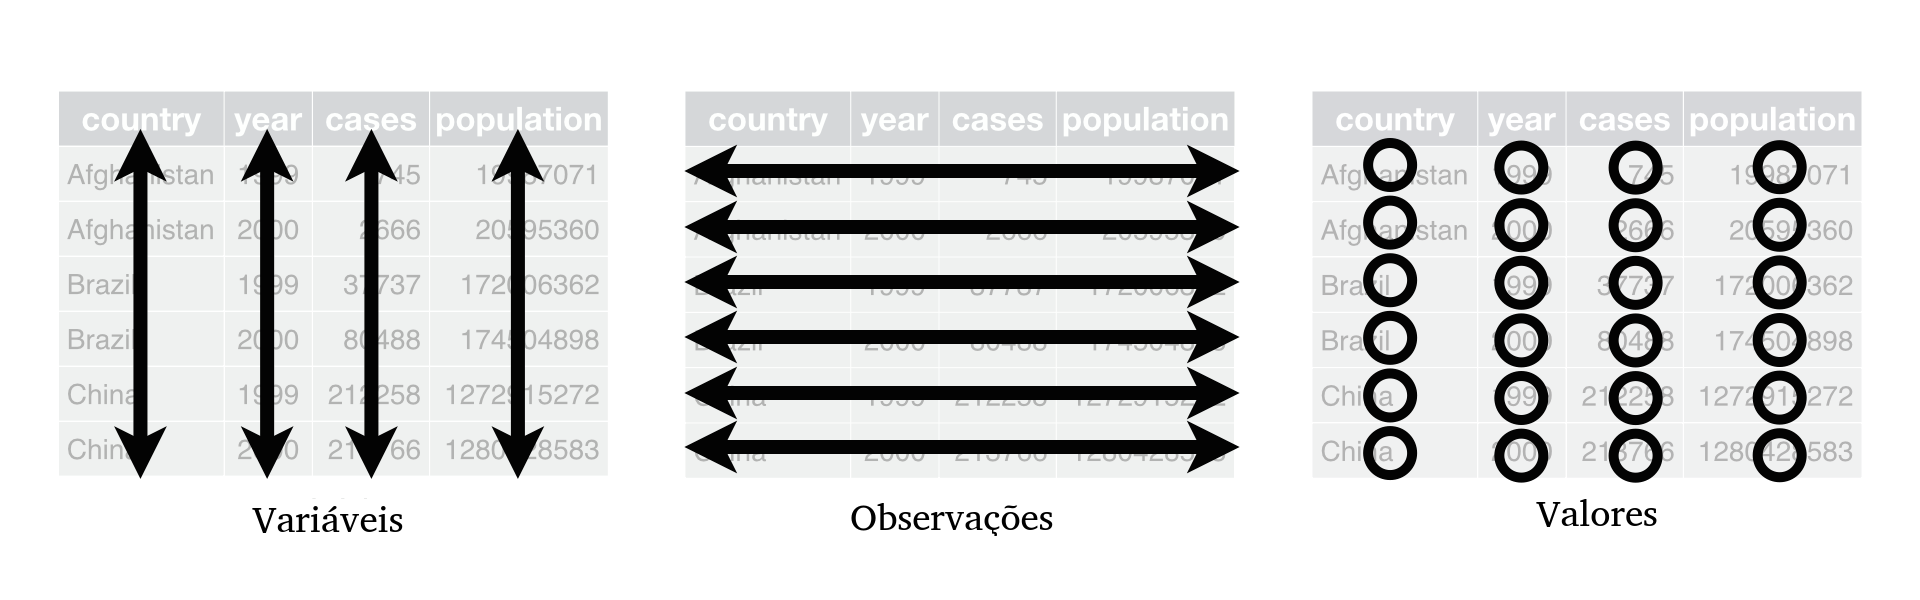
\includegraphics[width=\textwidth]{img/tidy-data_t.png}

\end{itemize}

\end{frame}

% -----------------------------------------------------------------

\section{Modelos de Regressão}

\begin{frame}[c, allowframebreaks]

\begin{itemize}
  
  \item Nos casos univariados mais gerais, estes modelos associam uma única variável resposta, a uma ou mais variáveis explicativas.

  \item De forma geral, um modelo de regressão é uma expressão matemática que relaciona a média da variável resposta às variáveis preditoras (covariáveis).
  
  \item A variável resposta segue uma distribuição de probabilidade condicional às covariáveis e a média é descrita por um preditor linear.

  \item Há casos em que são coletadas mais de uma resposta por unidade experimental e há o interesse de modelá-las em função de um conjunto de variáveis explicativas.
  
  \item Saímos então do cenário univariado (apenas uma resposta) e passamos para o multivariado (mais de uma resposta).
  
\end{itemize}

\framebreak 

São uma das principais e mais difundidas ferramentas utilizadas em diversas áreas do conhecimento, sendo comum o interesse em:

\begin{itemize}
  \item Explicar a associação entre uma variável resposta e um conjunto de variáveis explicativas.
  
  \item Utilizar o modelo para realizar predições para uma população.
\end{itemize}

\framebreak

Existem inúmeras classes de modelos de regressão:

\begin{itemize}
 \item Modelo Linear Normal.
 \item Modelos Lineares Generalizados (GLM).
 \item Modelos de regressão local.
 \item Modelos de regressão de splines.
 \item Modelos aditivos generalizados (GAM).
 \item Modelos de efeitos aleatórios.
 \item Modelos Aditivos Generalizados para Locação, Escala e Forma (GAMLSS).
 \item Modelos de regressão multivariados.
 \item Modelos Multivariados de Covariância Linear Generalizada (McGLM)
\end{itemize}


\end{frame}

% -----------------------------------------------------------------

\section{McGLM}

\begin{frame}[c, allowframebreaks]

\begin{itemize}
  \item Os GLMs são uma forma de modelagem univariada para dados de diferentes naturezas, tais como dados contínuos simétricos e assimétricos, contagens, dentre outras. 
  \item Tais características tornam essa classe de modelos uma flexível ferramenta de modelagem aplicável a diversos tipos de problemas.
\end{itemize}

Contudo, por mais flexível e discutida na literatura, essa classe apresenta duas principais restrições: 

\begin{enumerate}
  \item A incapacidade de lidar com observações dependentes.
  \item A incapacidade de lidar com múltiplas respostas simultaneamente.
\end{enumerate}

\framebreak

Com o objetivo de solucionar esses problemas, foi proposta uma estrutura geral para análise de dados denominada Modelos Multivariados de Covariância Linear Generalizada (MCGLM).

Esta classe de modelagem comporta:
\begin{itemize}
  \item Múltiplas respostas.
  \item Respostas de diferentes naturezas.
  \item Respostas correlacionadas.
  \item Observações não independentes.
  \item Extensões multivariadas para modelos de:
    \begin{itemize}
      \item Séries temporais.
      \item Dados longitudinais.
      \item Dados espaciais.
    \end{itemize}

\end{itemize}

\end{frame}

% -----------------------------------------------------------------

\section{MANOVA}

\begin{frame}[c, allowframebreaks]

A MANOVA clássica é um assunto com vasta discussão na literatura e possui diversas propostas com o objetivo de verificar a nulidade conjunta dos parâmetros de um modelo de regressão multivariado, como: 

\begin{itemize}
  \item Lambda de Wilk’s.
  \item Traço de Hotelling-Lawley.
  \item Traço de Pillai.
  \item Maior raiz de Roy.
\end{itemize}


Para o McGLM (cenário com múltiplas respostas não gaussianas) não existia teste similar. No trabalho:

\begin{itemize}
  \item Propomos e implementamos o teste de Wald para análise de variância multivariada para dados não gaussianos.
  \item Discutindo as propriedades e comportamento do teste proposto com base em estudos de simulação e aplicação a conjuntos de dados reais.
\end{itemize}

\end{frame}

% -----------------------------------------------------------------

\section{Proposta para o mestrado}

\begin{frame}[c, allowframebreaks]

A proposta incial era:

\begin{itemize}
  \item Construção de outros testes multivariados para dados não gaussianos no contexto dos MCGLMs.
  \item Ampliar o estudo de simulação, de forma a considerar cenários não abrangidos.
  \item Encontrar formas de melhorar o tempo computacional dos estudos de simulação. 
\end{itemize}

\framebreak

Proposta atual:

\begin{itemize}
  \item Artigo 1: reimplementar o pacote car com foco em objetos mcglm.
    \begin{itemize}
      \item Diferentes tipos de output.
      \item Gráficos.
      \item Testes de comparações múltiplas.
      \item Etc.
    \end{itemize}

  \item Artigo 2: estudo de simulação.
    \begin{itemize}
      \item Simular o maior número de casos possíveis de conjuntos de dados.
      \item Ajustar o modelo para cada um deles, aplicar o teste e reportar em que casos o teste funcionou ou não.
      \item Verificar como as revistas fazem para simular coisas do tipo.
    \end{itemize}
    
  \item Artigo 3: Analisar conjuntos de dados reais.
    \begin{itemize}
      \item Ajustar o modelo.
      \item Aplicar o teste proposto.
      \item Reportar os resultados.
    \end{itemize}
\end{itemize}

Fica na lista de afazeres propor e implementar os outros testes porque é um caminho muito nebuloso.

\framebreak

Considerando o grupo de pesquisa (Data Science \& Big Data) o trabalho teria as seguintes contribuições:

\begin{enumerate}
  \item Propor um teste novo para uma classe de modelos não usual mas com alto potencial de aplicação.
  \item Realizar um estudo pesado de simulação para verificar o funcionamento do teste proposto.
  \item Análise de dados.
\end{enumerate}

\framebreak

\begin{figure}[t]
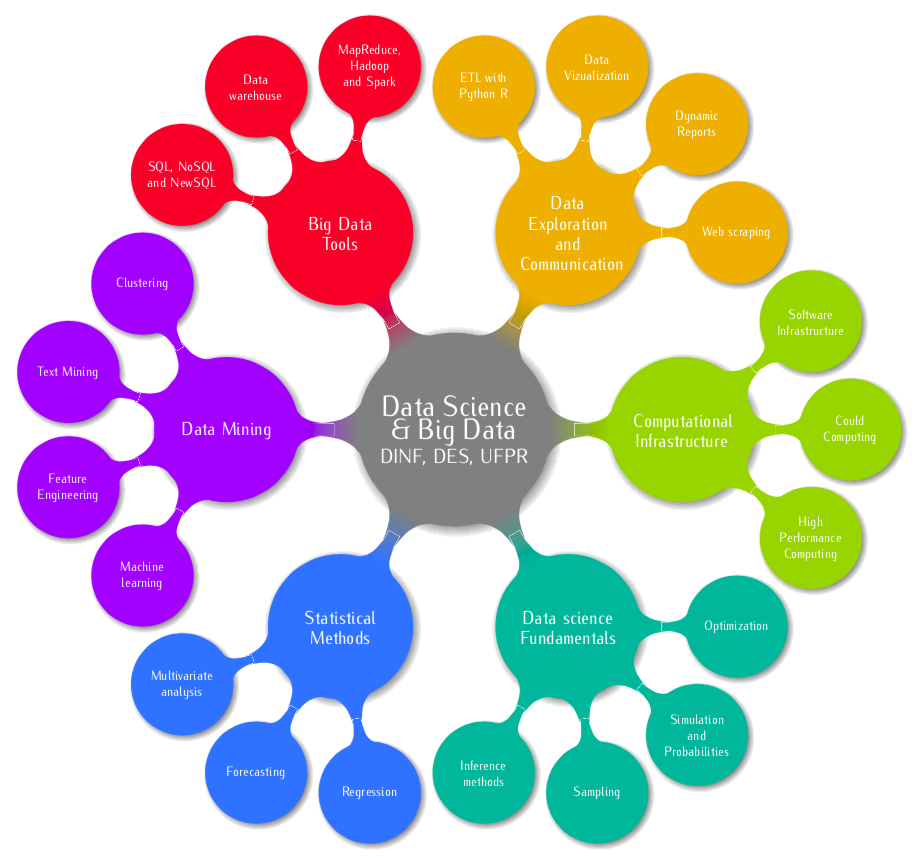
\includegraphics[width=7.5cm, height=7.5cm]{img/dsbd2_t.png}
\centering
\end{figure}



\end{frame}


\end{document}
